\section{Implementation 1}
The PyBullet environment for testing this design consists of a table, soft ball and a robotiq 140 gripper Fig \ref{fig:pybullet_env_design_one}. The table and gripper were imported using a Unified Robot Description Format (URDF) an XML-based file format used to describe the physical and kinematic properties of a robot. The soft ball was created using open source 3D moddeling software - Blender. The blender file exported as .obj provides only the surface mech. To obtain volumetric mesh needed to simulate the soft body, open source software - GMSH was used. 

\begin{figure}[ht]
  \centering
  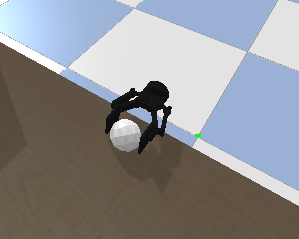
\includegraphics[width=0.4\linewidth]{chapters/exoskeleton/images/background/pybullet_design_one_minimal_setup.png}
  \caption{PyBullet environment for testing \nameone}
  \label{fig:pybullet_env_design_one}
\end{figure}

\bigskip \noindent
The gripper has stroke range of 0 to 0.127 units in the simulation. It is controlled by a single motor using position control. A function that controls the robotiq gripper based on distance instead of angle was created by linearly spacing 100 points of gripper's stroke range, measuring the angle of the motor and the distance between the fingerpads in simulation and fitting this data using a polynomial Fig \ref{fig:robotiq_polynomial_fit}.

\begin{figure}[ht]
  \centering
  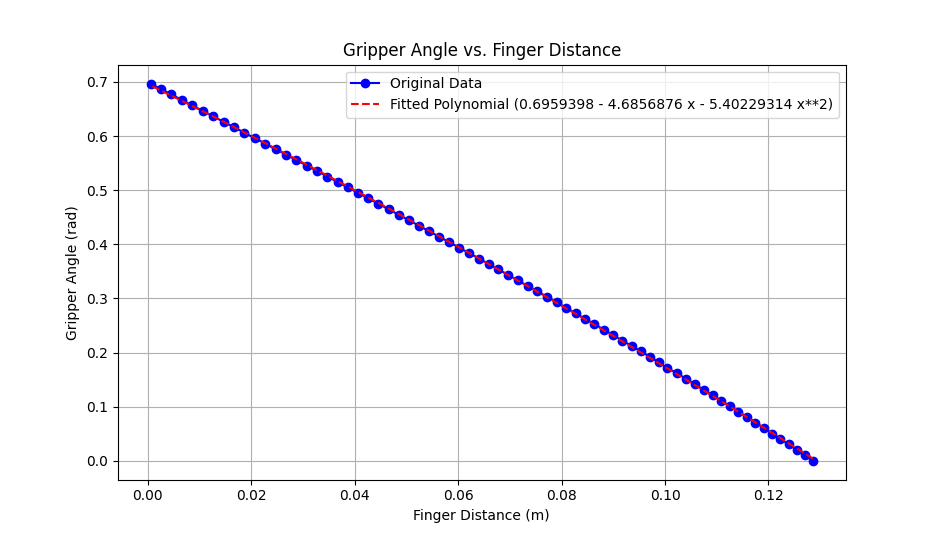
\includegraphics[width=0.8\linewidth]{chapters/exoskeleton/images/background/polynomial_fitting_robotiq.png}
  \caption{Polynomial fitting of data between gripper's motor angle and distance between finger pads}
  \label{fig:robotiq_polynomial_fit}
\end{figure}

\bigskip \noindent
The Dynamixel motors are controlled with the python files provided in their SDK.
The distance between finger pads can be calculated using simple trigonometry Eq \ref{eq:trigonometry_distance_prototype1}, Fig \ref{fig:trigonometry_distance_prototype1}. This distance obtained from the motors is scaled and applied to the simulation every frame.

\begin{equation}
  \label{eq:trigonometry_distance_prototype1}
  \begin{aligned}
      p_1 &= r_1 \cdot \cos(a_1) \\
      p_2 &= r_2 \cdot \cos(a_2) \\
      d_{total} &= -p_1 + d_0 + p_2 
  \end{aligned}
\end{equation}

\begin{figure}[ht]
  \centering
  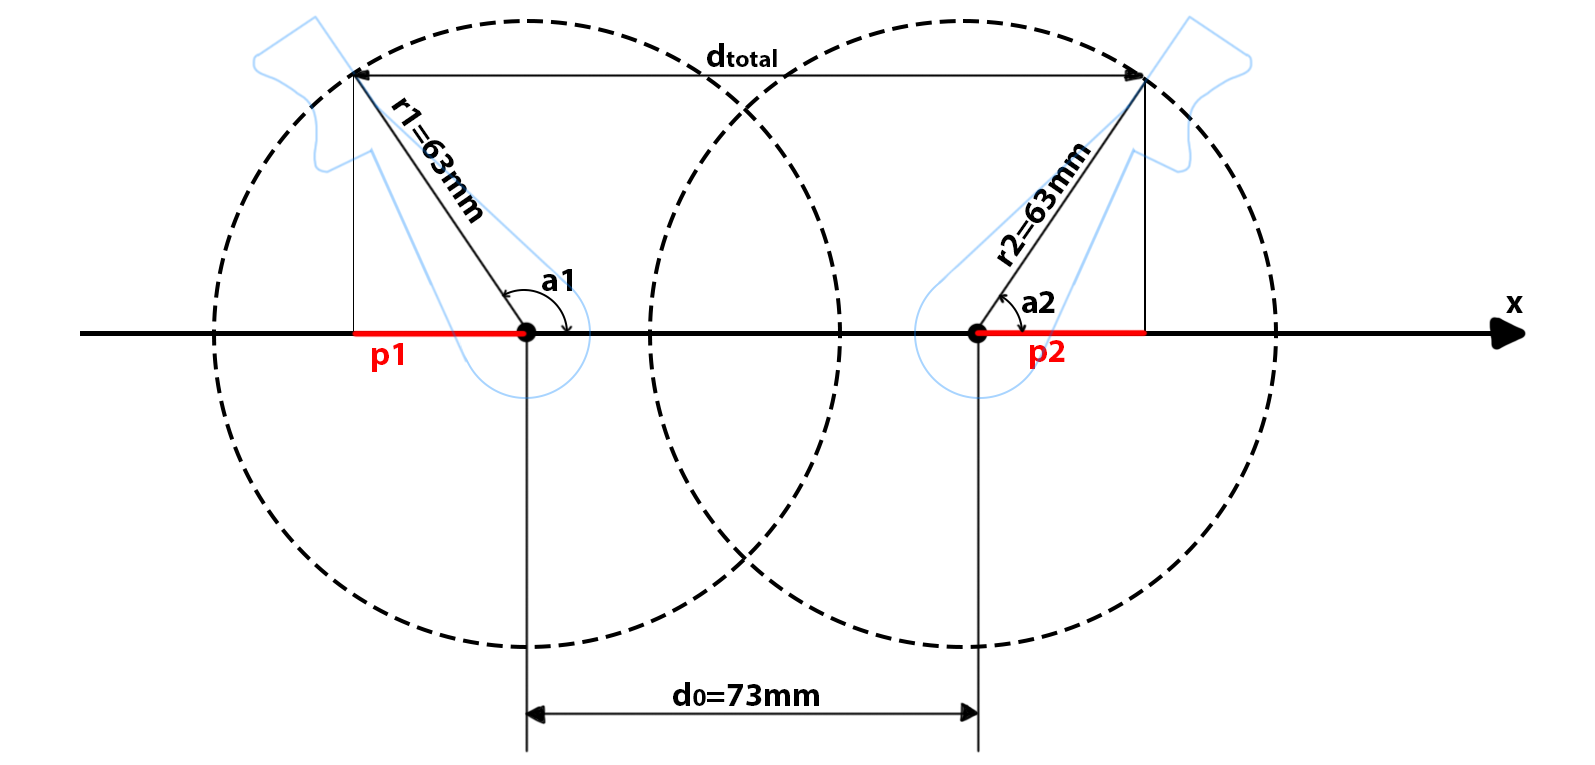
\includegraphics[width=0.8\linewidth]{chapters/exoskeleton/images/background/prototype1_trigonometry.png}
  \caption{Diagram of distance calculation for \nameone}
  \label{fig:trigonometry_distance_prototype1}
\end{figure}

\bigskip \noindent
The PyBullet's Neo-Hookean model was used for soft-body simulation. While linear models like Hooker's Law can be used to model small strains, materials that undergo large deformations need to use a hyperelastic model that account for their nonlinearities. Neo-Hookean is a simple form of hyperelastic model. It is characterized by strain energy density function, which defines the energy stored in the material due to deformation. The Neo-Hookean model decouples this energy into two parts, deviatoric that handles shear deformations and volumetric part that deals with volume changes. The model is configured by material dependant Lamé parameters that describe the mechanical behavior of isotropic solids. The first Lamé parameter $\lambda$ is related to the volumetric changes and the second Lamé parameter (shear modulus) $\mu$ is used to describe the material’s resistance to shear deformation. Both of these parameters can be calculated \cite{febio2023} from material properties E (Young’s modulus) and $\nu$ (Poisson’s
ratio) Eq \ref{eq:lame_parameter_mu}, \ref{eq:lame_parameter_lambda}.

\begin{equation}
  \label{eq:lame_parameter_mu}
  \mu = \frac{E}{2(1 + \nu)}
\end{equation}

\begin{equation}
  \label{eq:lame_parameter_lambda}
  \lambda = \frac{E \nu}{(1 + \nu)(1 - 2\nu)}
\end{equation}

\noindent
A study \cite{10637182} has shown that it is possible predict these parameters using data driven model to accurately simulate real world soft models in PyBullet. It also mentions that soft-bodies tend to become unstable (implode or explode) when Lamé parameters are set too low or to high. Another reason for soft-body instability is that the simulation is run in discrete time steps, the lack of fidelity can cause numerical issues during sudden application of large forces. Some solvers use adaptive time stepping to overcome this issue, but such feature is unavailable in PyBullet. It's a common practice to set PyBullet's time step to 1/250 of a second, but this value turned out to have poor stability during the experiments. A value of 1/1000 was used as it yielded much better stability. Another factor that influenced stability was the mesh itself.  Multiple balls were created using icosphere mesh with varying subdivision setting Fig \ref{fig:ball_subdivissions}. Increasing subdivisions increases the resolution of the mesh, making the ball appear smoother, but it also increases the vertex count potentially making soft body simulation unstable or slower. A ball with 2 subdivissions was used as it yielded the best performance and stability.


\begin{figure}[ht]
  \centering
  \begin{subfigure}{0.3\textwidth}
      \centering
      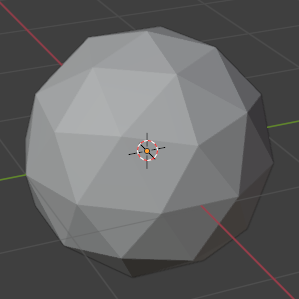
\includegraphics[width=\textwidth]{chapters/exoskeleton/images/implementation/cropped-2_subdivissions.png}
      \caption{2 subdivision}
  \end{subfigure}
  \begin{subfigure}{0.3\textwidth}
      \centering
      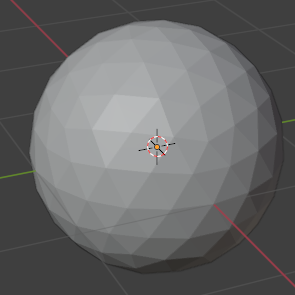
\includegraphics[width=\textwidth]{chapters/exoskeleton/images/implementation/cropped-3_subdivissions.png}
      \caption{3 subdivissions}
  \end{subfigure}
  \begin{subfigure}{0.3\textwidth}
      \centering
      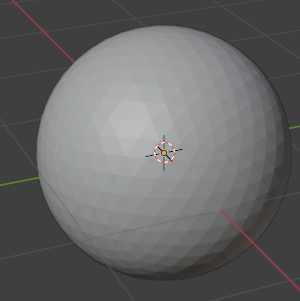
\includegraphics[width=\textwidth]{chapters/exoskeleton/images/implementation/cropped-4_subdivissions.png}
      \caption{4 subdivissions}
  \end{subfigure}
  \caption{Varying subdivission setting}
  \label{fig:ball_subdivissions}
\end{figure}

\bigskip \noindent
The normal forces between soft ball and gripper pads are obtained using PyBullet's function getContactPoints. The reaction forces $Rl$ and $Rr$ in PyBullet are assumed to be distributed symetrically and can be represented with total resultant force as a sum of individual forces at the centroid of the contact area. In order to achieve the force feedback in the exoskoleton, the reaction forces from simulation are converted to motor torques Eq \ref{eq:motor_reaction_torques}


\begin{equation}
  \label{eq:motor_reaction_torques}
  \begin{aligned}
      \tau_l &= R_l d_l sin\theta \\
      \tau_r &= R_r d_r sin\theta
  \end{aligned}
\end{equation}

where:  
\begin{itemize}
    \item \( \tau \) is the motor torque required to exhert equivalent reaction force,
    \item \( R \) is the equivalent normal reaction force,
    \item \( d \) is the distance between the reaction force and the center of rotation,
    \item \( \theta \) is the angle between force and the lever arm.
\end{itemize}


\begin{figure}[ht]
  \centering
  \begin{subfigure}{0.45\textwidth}
      \centering
      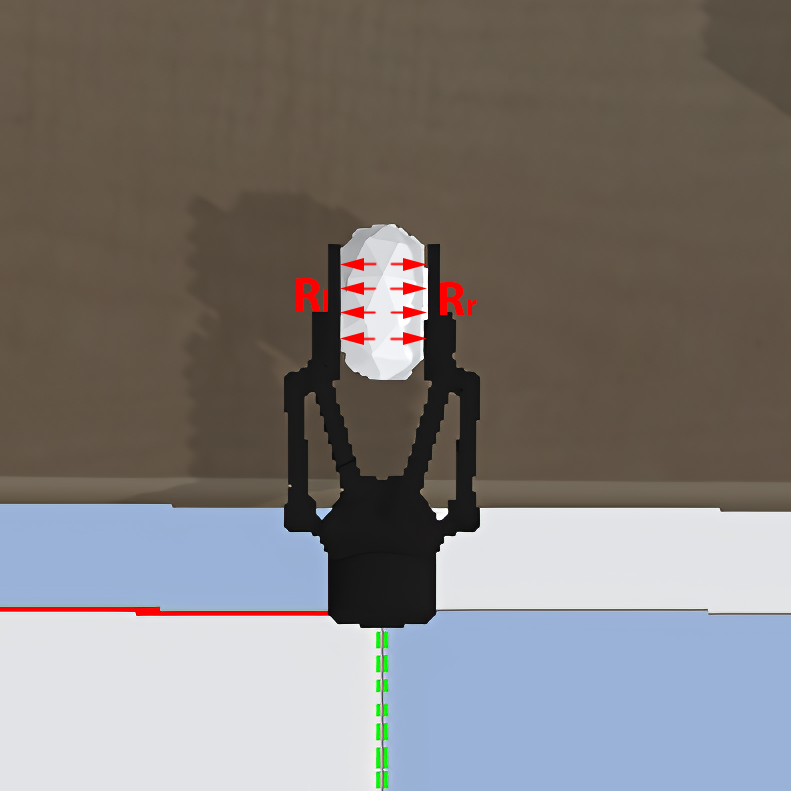
\includegraphics[width=\textwidth]{chapters/exoskeleton/images/implementation/squeezing ball.png}
      \caption{Force diagram PyBullet}
      \label{fig:pybullet_getContactPoints}
  \end{subfigure}
  \begin{subfigure}{0.45\textwidth}
      \centering
      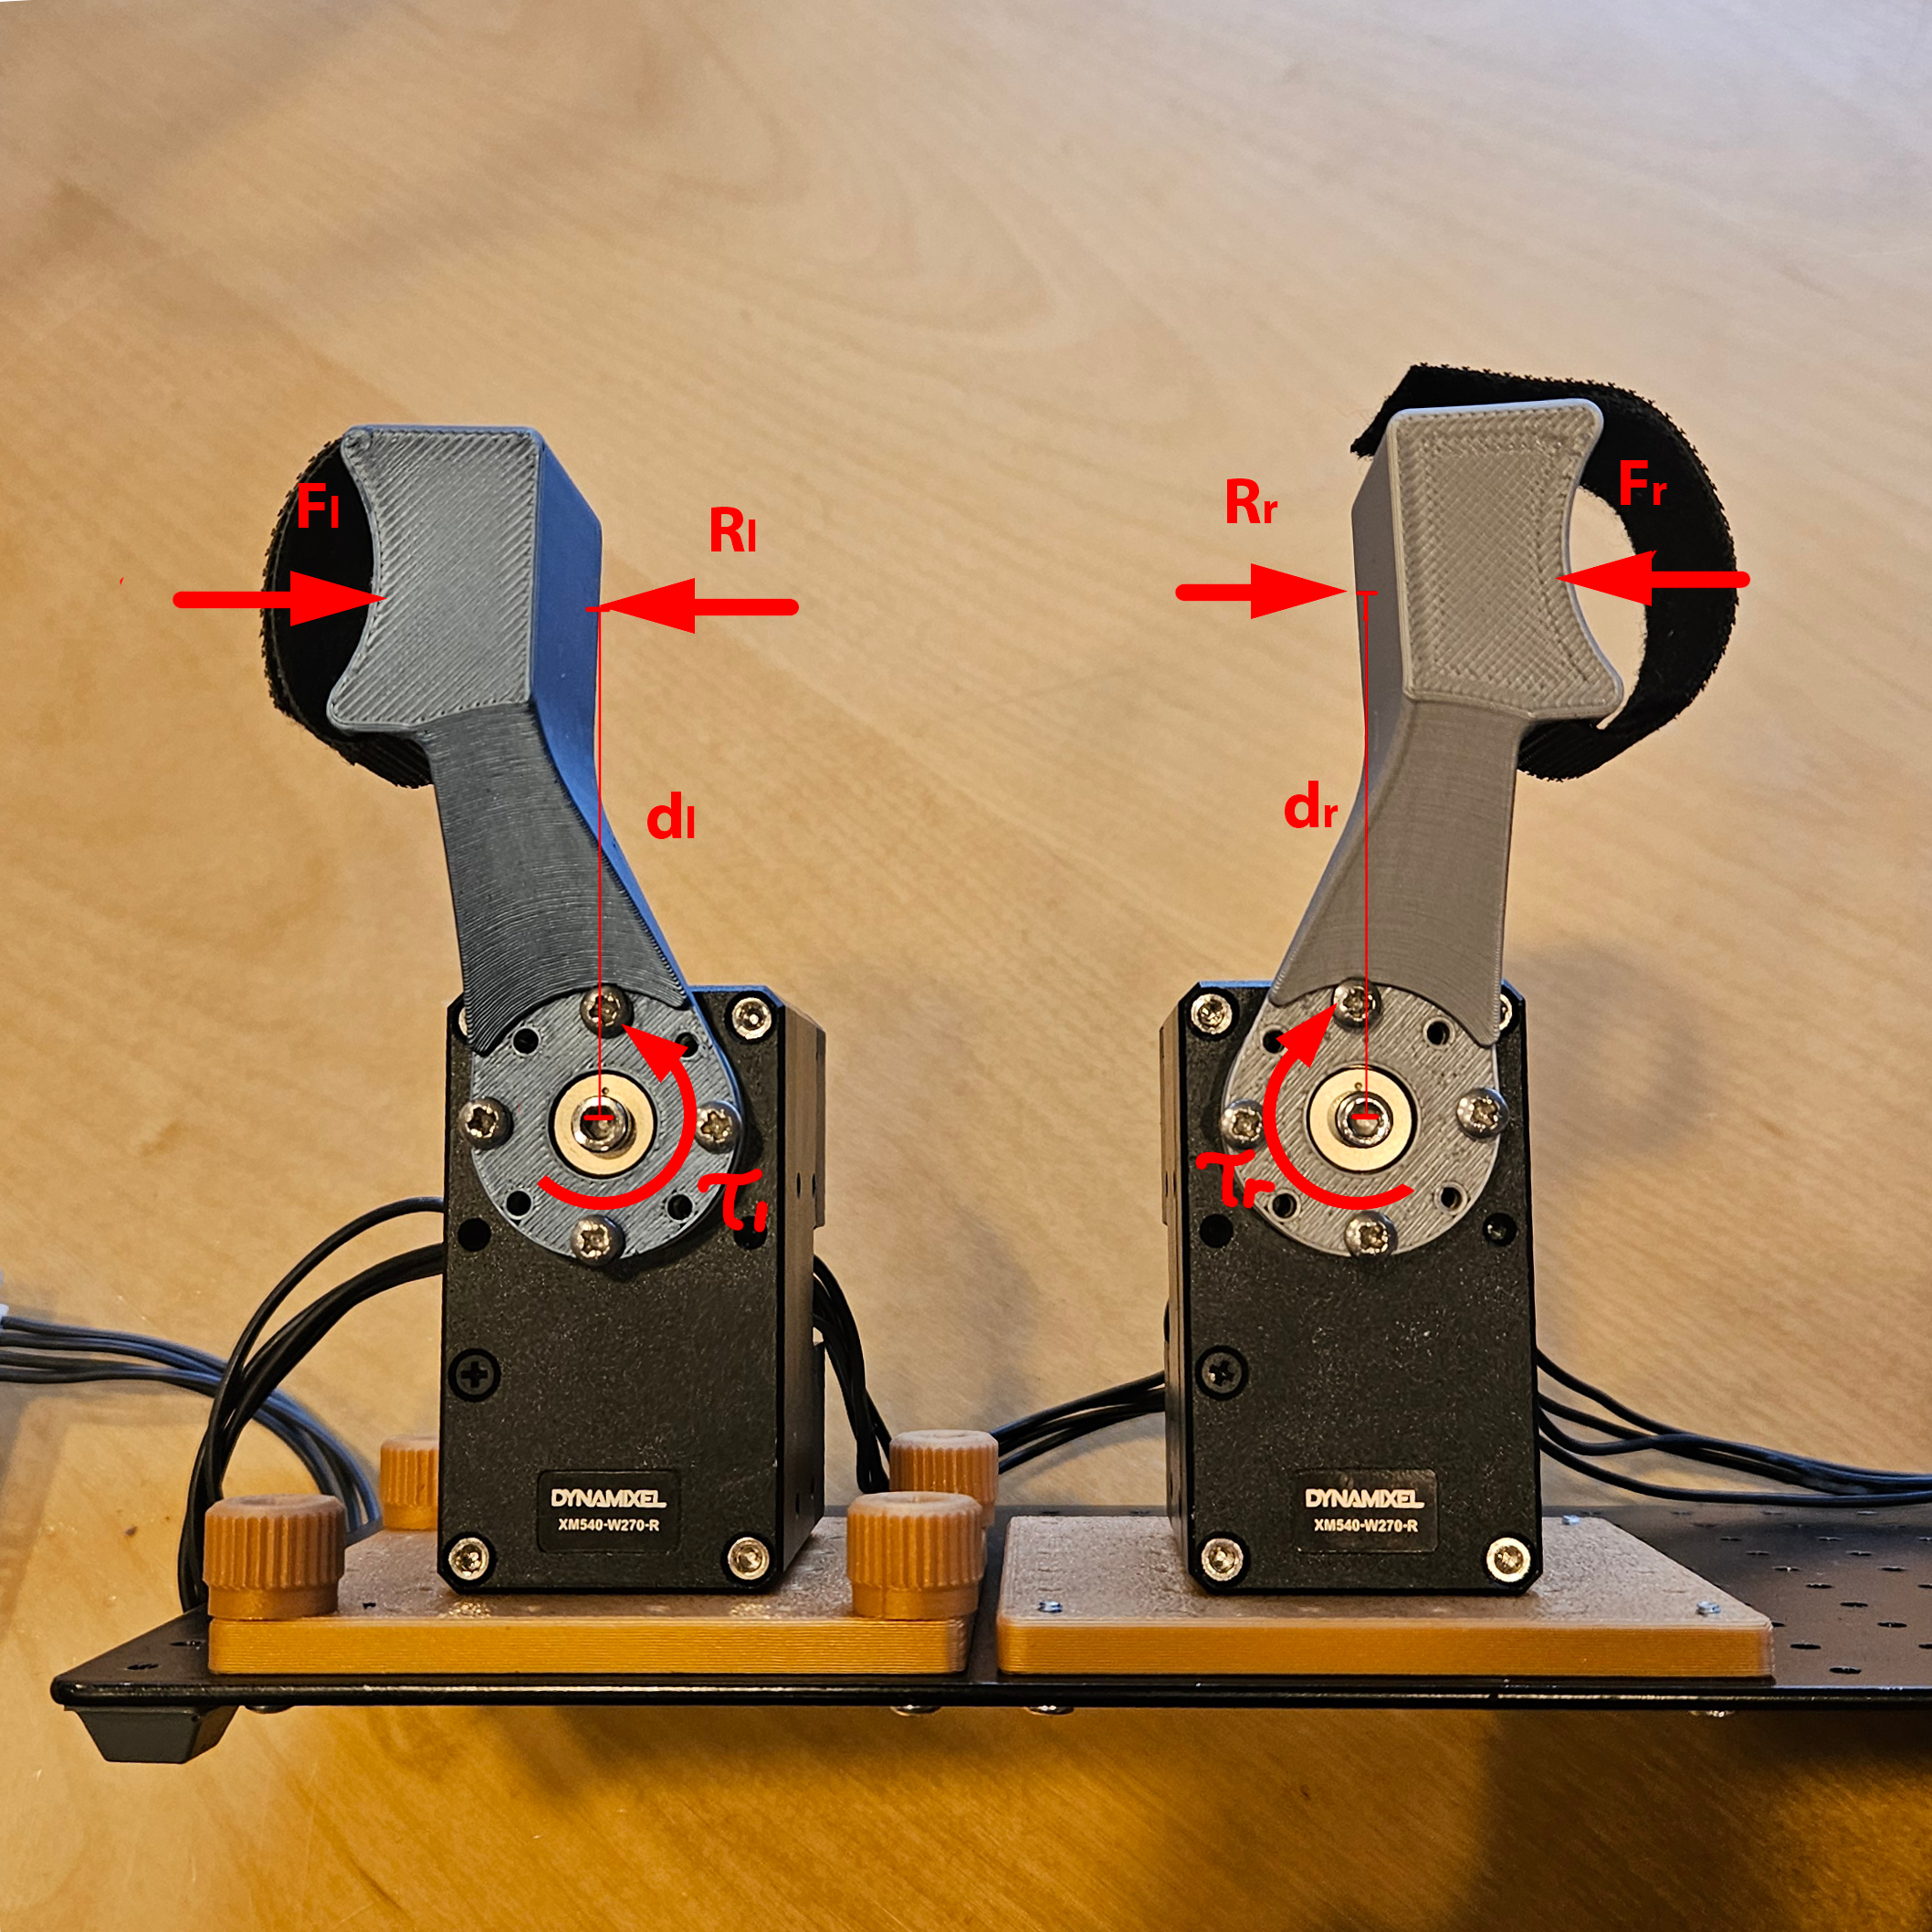
\includegraphics[width=\textwidth]{chapters/exoskeleton/images/implementation/motor_torque.png}
      \caption{Force diagram \nameone}
  \end{subfigure}
  \caption{Force diagrams}
  \label{fig:forces_diagram}
\end{figure}

\bigskip \noindent
XM540-W270-T/R are smart servo motors; they have several control modes available: Current Control Mode,
Velocity Control Mode,
Position Control Mode (0 360 [°]) and
PWM Control Mode (Voltage Control Mode). The current control mode and PWM control mode could both be suitable in this scenario, so they will be tested and comparison between them will be made. 

\subsection{PWM control}
The Pulse Width Modulation (PWM) is a low level motor control mode and is the final step in all of the control modes. It can give fine grain control over the motors if the available control modes are not satisfactory. Additionally, not all motors provide multiple control modes, it is common for direct current (DC) motors to only use PWM control as a means to change the speed of the motor. PWM signal is a square wave with the signal either being on (set to the maximum voltage) or off (zero voltage). The average voltage delivered to the motor depends on the duty cycle, a ratio of the "on" time to the total period of the signal. For the motor used $PWM \in \mathbb{Z} \cap [-885, 885]$, where 0 would be duty cycle 0\%, 885 duty cycle  100\% in counter clock wise (CCW) direction and -885 duty cycle 100\% in clock wise (CW) direction.

\begin{equation}
  \label{eq:duty_cycle}
  V_{out} = V_{max} \cdot DutyCycle
\end{equation}

\bigskip \noindent
The motor torque holds a linear relationship to the supplied current Eq \ref{eq:current}, where $k_t$ is torque constant. From the XM540-W270-T/R motor's datasheet, we can see that stall torque is 10.6 [Nm] (at 12.0 [V], 4.4 [A]). Using this information the torque constant can be calculated: $k_t = \tau / I = 10.6 / 4.4 = 2.409 $

\begin{equation}
  \label{eq:current}
  \tau = k_t \cdot I
\end{equation}

\bigskip \noindent
The motor can measure the supplied current, thus the goal of PWM control will be to reach and maintain a goal current instead of torque as the value can be converted back to the torque later on. The PID controller diagram can be seen in Fig \ref{fig:PID_controller}, the motor's servo arm is placed against a fixed support, once the PWM signal is set, the reaction force from the fixed support generate resistance that is measured by the motor in form of current. 

\begin{figure}[ht]
  \centering
  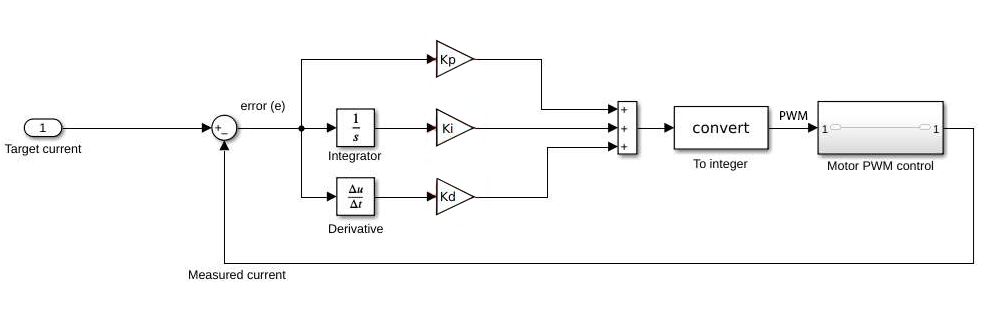
\includegraphics[width=\linewidth]{chapters/exoskeleton/images/implementation/PID_control.png}
  \caption{Diagram of PID controller}
  \label{fig:PID_controller}
\end{figure}

\bigskip \noindent
The Kp, Ki and Kd gains need to be tuned. When the transfer function is known, analytical methods such as root locus could be used to tune a PID controller to meed performance requirements. However, for model-free systems, manual tuning is commonly employed, or heuristic approaches like Ziegler–Nichols can be used to obtain initial controller parameters. Manual tunning was employed, but it proved to be difficult and time consuming. It was also very easy to get stuck in a local minima as drastic changes in gains require to restart tuning process. During this trial and error phase an interesting idea occured to me. By employing evolutionary algorithm (EA), variety of gains could be tested autonomously based on desired fitness function. When the ball in simulation is squeezed the reaction forces and thus the target currents will be changing rapidly. Intuitively, a good fitness function should encompass rapid changes. For this reason a target current is chosen as a step function Eq \ref{eq:test_ga} and the fitness of the individuals will be a sum of absolute errors, meaning the best performing members of the population will be able to reach the target signal with minimal rise time and steady state error.

\begin{equation}
  f(\text{iteration}) =
  \begin{cases}
  0.2 & \text{if } 600 < \text{iteration} < 1200 \\
  0.1 & \text{otherwise, where iteration} \leq 1800
  \end{cases}
  \label{eq:test_ga}
\end{equation}

\bigskip \noindent
A population of size 150 was initialized. Each member was assigned random P,
I, and D values in ranges [0, 1024], [0, 512], and [0, 64], respectively. The algorithm was trained for 20 generations with a mutation rate of 0.1. The top-performing member of the population has the PID values Kp = 28.809, KI =
503.211, and KD = 0.191 with the fitness value of 2.295. This is a significant improvement as the fitness for a manually tunned controller is 8.824. 

\bigskip \noindent
After the training the PID controller was tested against a more varied target function that includes triangle and sinusoidal waves Fig \ref{fig:ga_testing_function}. The controller is able to follow the target quite well, the fitness for this function is 54.8. On average in the testing function the present current is delayed by 17 iterations, which equites to 131.059ms with average iteration time being 7.709ms

\begin{figure}[ht]
  \centering
  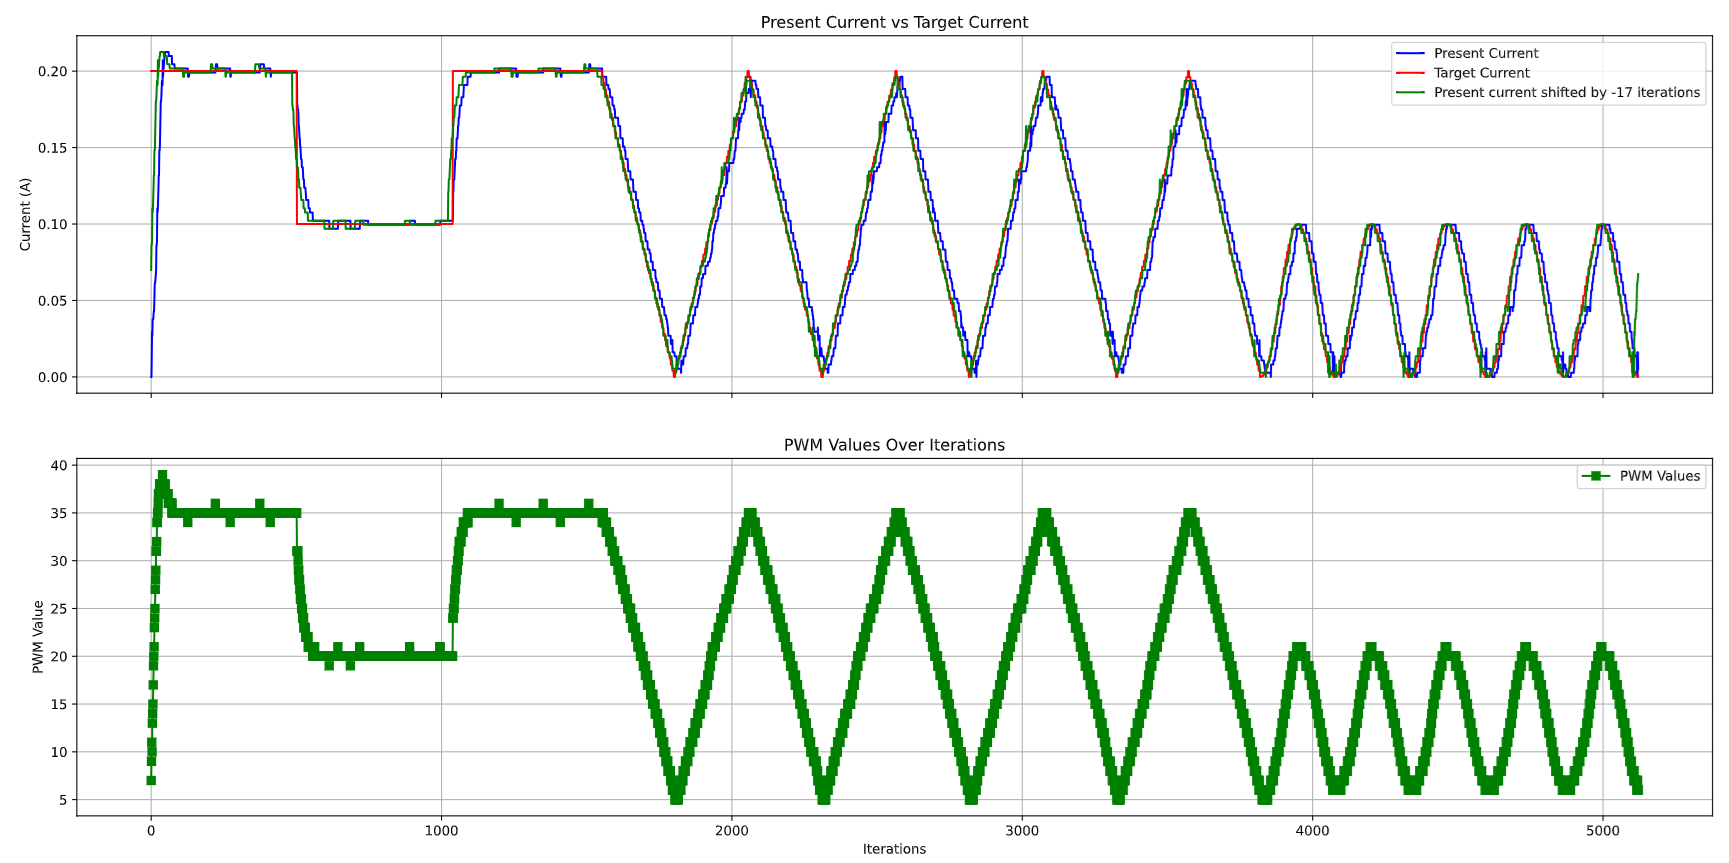
\includegraphics[width=\linewidth]{chapters/exoskeleton/images/genetic_algorithm/testing_ga.png}
  \caption{Function for testing trained PID values}
  \label{fig:ga_testing_function}
\end{figure}

\bigskip \noindent
The exoskeleton was also tested by squeezing the virtual ball. The sensation subjectively feels convincing, but looking at the Fig \ref{fig:ga_squeeze_ball} it is evident that the significant delay in reaching target current results in a discrepancy between the forces accoring to the simulation and forces that are felt. Note that the controller is disengaged when the target current is zero, otherwise the PWM controller generates resistance instead of being in freewheeling condition.

\begin{figure}[ht]
  \centering
  \begin{subfigure}{\textwidth}
    \centering
  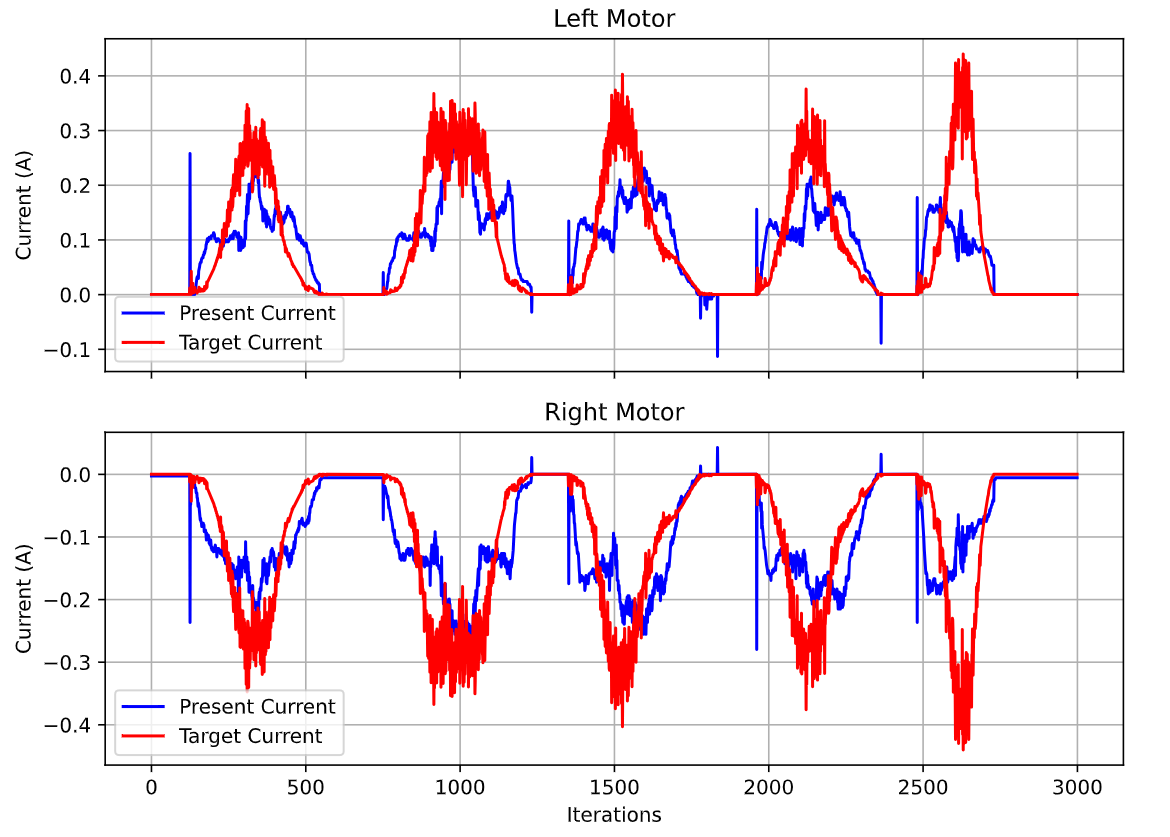
\includegraphics[width=0.7\linewidth]{chapters/exoskeleton/images/genetic_algorithm/testing_ball_switching.png}
  \caption{Current}
  \end{subfigure}
  \centering
  \begin{subfigure}{\textwidth}
    \centering
    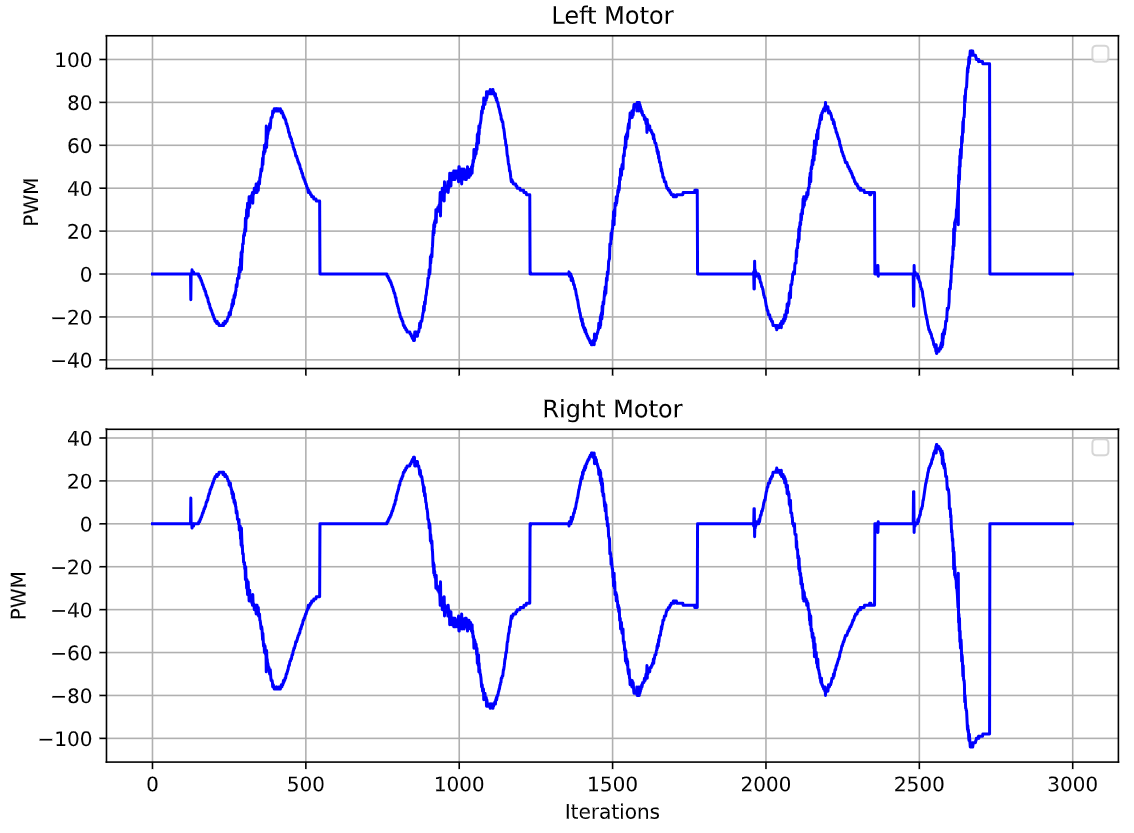
\includegraphics[width=0.7\linewidth]{chapters/exoskeleton/images/genetic_algorithm/testing_pwm_switching.png}
    \caption{PWM}
  \end{subfigure}
  \caption{Squeezing the virtual ball 5 times using PWM control}
  \label{fig:ga_squeeze_ball}
\end{figure}

\subsection{Current control}
This control mode allows the current to be controlled directly. Internally it works similarly to the controller we have implemented in the section above. As seen in Fig \ref{fig:current_control_test} when tested, this controller has a much better performance compare to out implemented PWM control, with fitness (sum of absolute errors) being 18.823 and reaching target current in less than 8ms (one iteration, exact time is unknown as this is as fast as we can measure). This performance can be attributed to Dynamixel having well-tuned PID loops optimized for their hardware and low latency feedback due to motor performing controlling internally without the need of slow communication and signal conversion to the PC.

\begin{figure}[ht]
  \centering
  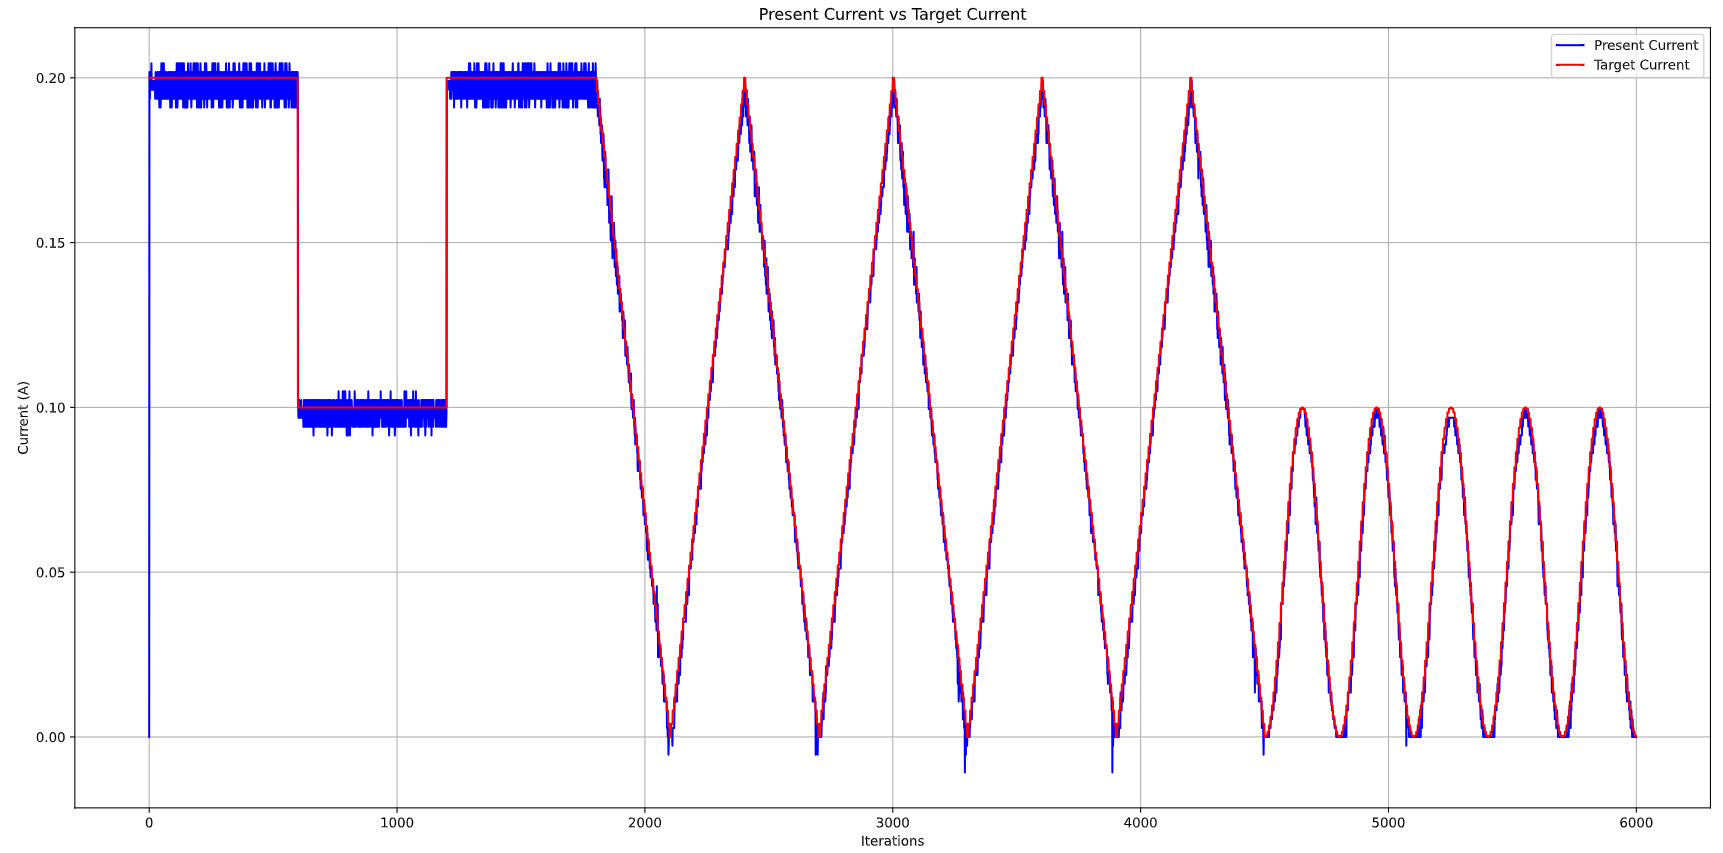
\includegraphics[width=0.7\linewidth]{chapters/exoskeleton/images/current/current_control.png}
  \caption{Current control test}
  \label{fig:current_control_test}
\end{figure}

\bigskip \noindent
When squeezing the virtual ball (Fig \ref{fig:current_control_5_times_squeeze}) we can see that the current is followed closely, but subjectively the experience does not feel smooth, rapid oscilations in target current occur. By taking a closer look to a single squeeze Fig \ref{fig:current_no_smoothing} we can see how uneven the target current is. This issues could be mitigated by processing the signal using exponential smoothing Eq \ref{eq:test_exponential_smoothing}. A variety of different window size values have been tested and plotted \ref{fig:exponential_smoothing_k_variations}. Increasing the window size provides smoother signal but adds a higher delay. For the controller a windows size of 10 is used as it provides a smoother signal without much delay \ref{fig:current_smoothing}. This controller still does struggle to maintain low target current when suddenly introduced with external forces from the fingers.

\begin{figure}[h!t]
  \centering
  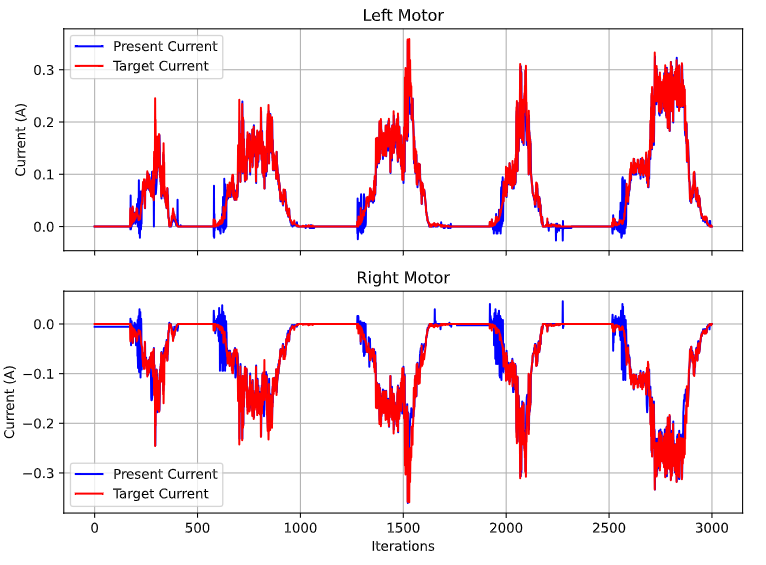
\includegraphics[width=0.7\linewidth]{chapters/exoskeleton/images/current/squeezing_ball_5_times.png}
  \caption{Squeezing the virtual ball 5 times using Current control}
  \label{fig:current_control_5_times_squeeze}
\end{figure}

\begin{figure}[h!t]
  \centering
  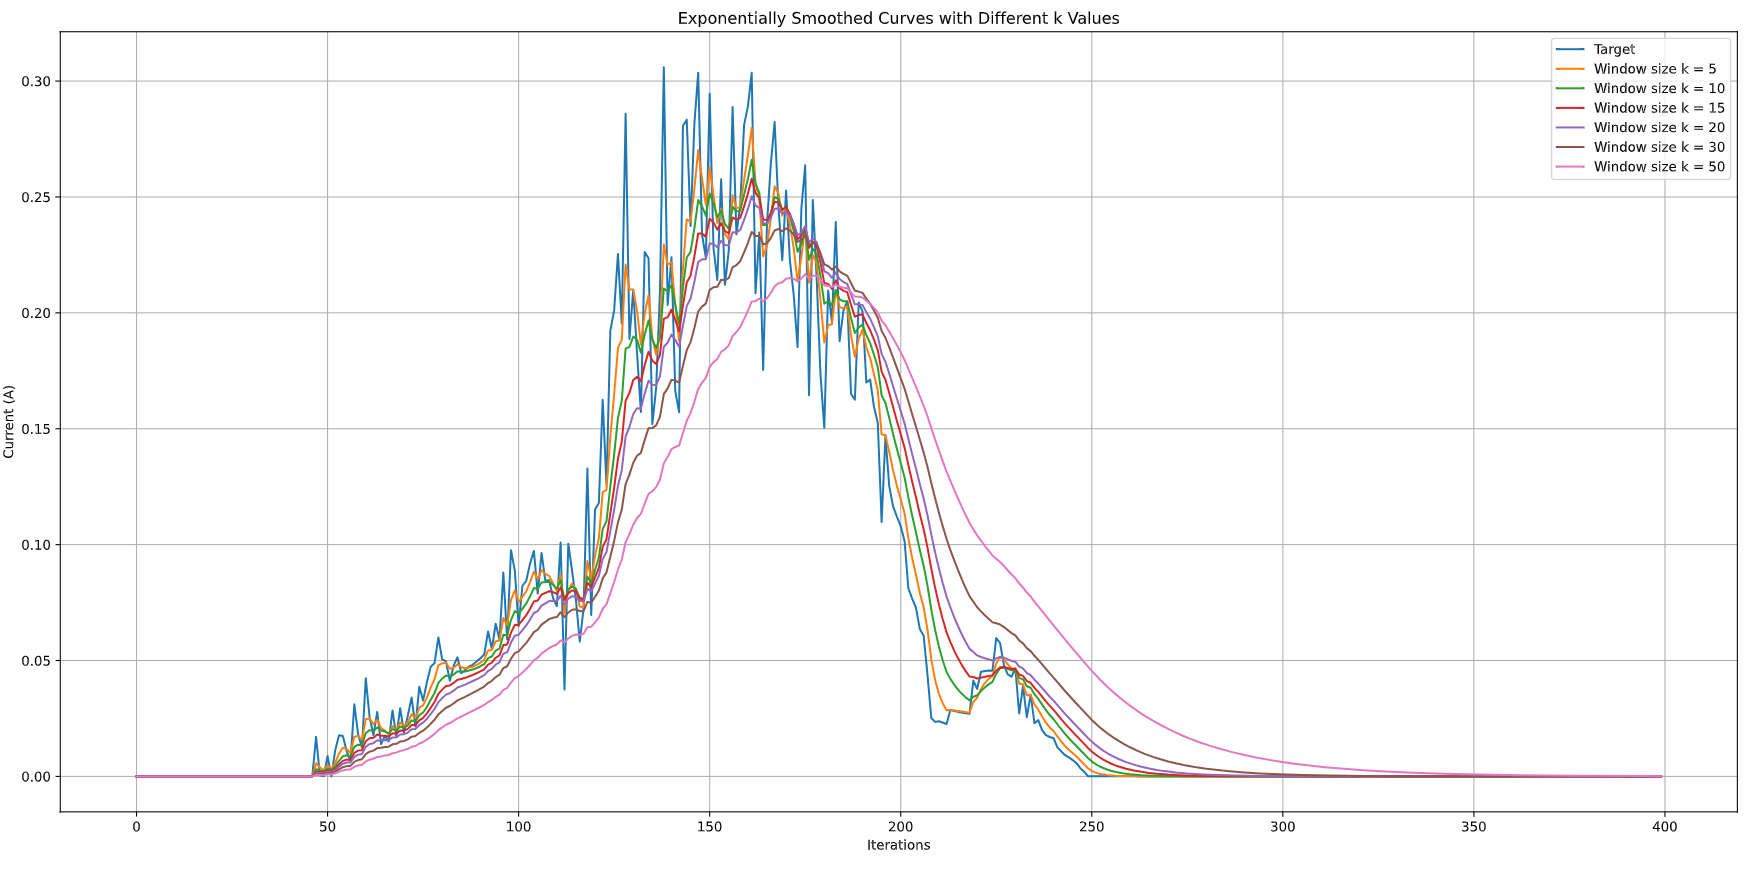
\includegraphics[width=0.7\linewidth]{chapters/exoskeleton/images/current/smoothed_curves.png}
  \caption{Exponential smoothing with different window sizes}
  \label{fig:exponential_smoothing_k_variations}
\end{figure}

\begin{figure}[h!t]
  \centering
  \begin{subfigure}{\textwidth}
    \centering
  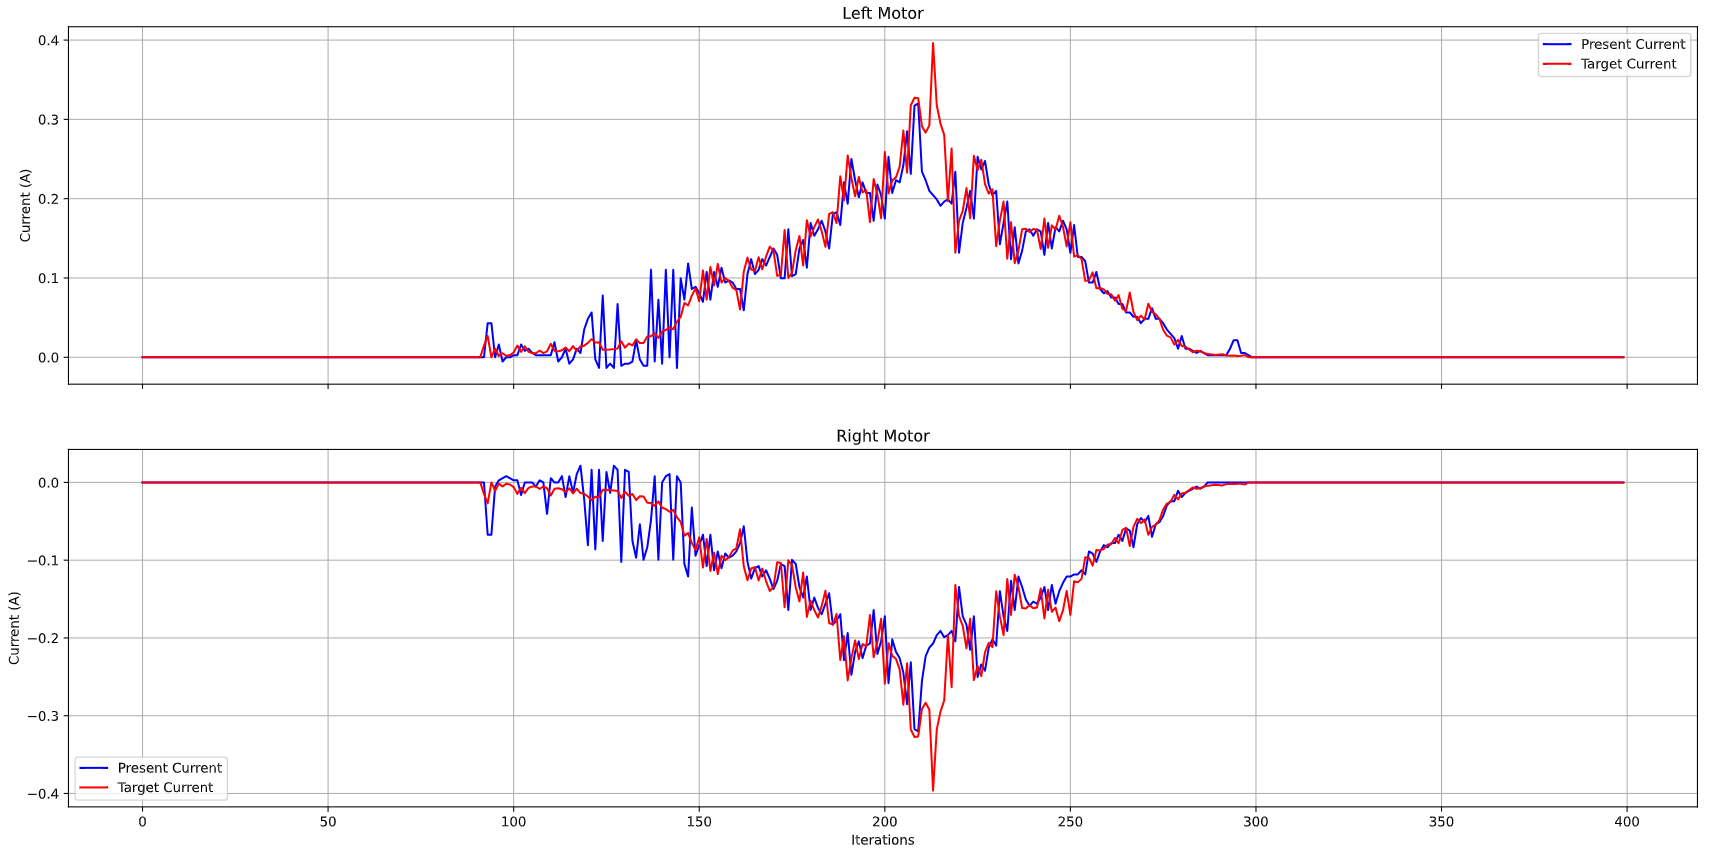
\includegraphics[width=0.7\linewidth]{chapters/exoskeleton/images/current/No_smoothing.png}
  \caption{No target current smoothing}
  \label{fig:current_no_smoothing}
  \end{subfigure}
  \centering
  \begin{subfigure}{\textwidth}
    \centering
    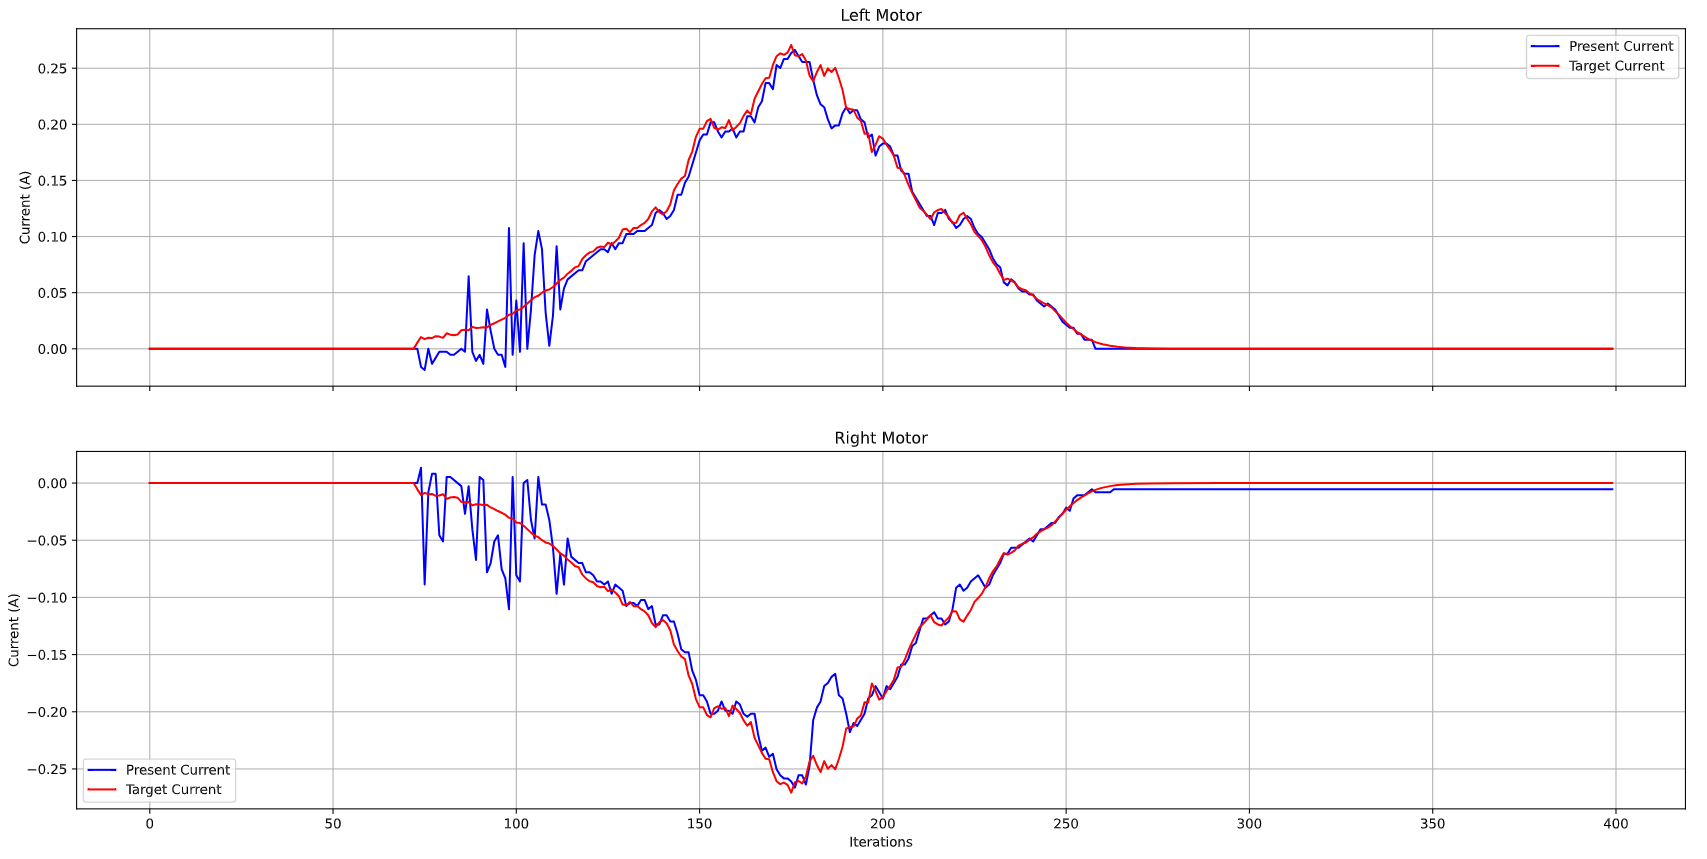
\includegraphics[width=0.7\linewidth]{chapters/exoskeleton/images/current/smoothing_k10.png}
    \caption{Target current exponential smoothing with K=10}
    \label{fig:current_smoothing}
  \end{subfigure}
  \caption{Influence of exponential smoothing when squeezing a virtual ball}
  \label{fig:current_smoothing_no_smoothing}
\end{figure}


\begin{equation}
  S_t = \alpha X_t + (1 - \alpha) S_{t-1}, \quad \text{where } \alpha = \frac{2}{K+1}
  \label{eq:test_exponential_smoothing}
\end{equation}

\noindent
where:  
\begin{itemize}
    \item \( S_t \) is the smoothed value at time \( t \),
    \item \( X_t \) is the actual value at time \( t \),
    \item \( \alpha \) is the smoothing factor, calculated using window size \( K \),
    \item \( S_{t-1} \) is the previous smoothed value.
\end{itemize}

